%BEGIN: DISCUSSION
\section{Discussions}\label{sec:discussions}

%Service in Smart Homes
The framework presented in Section \ref{sec:services_in_smart_homes} is solely oriented towards emulating sensors withing a smart home. The system supports in the simulated environment both emulated sensors and representation of real-life sensory data. For the implementation of virtual stubs they have employed the service-oriented computing paradigm, which is widely used to implement systems requiring high interoperability, scalability, security and reliability. One of the main advantages is that such software can seamlessly integrate other systems written in other programming languages and even deployed under different operating systems.\\

Although they have created a highly decoupled architecture, the framework is able to represent a very limited types of entities. The characteristics monitored by the framework for the entities and the simulated agent are limited to proximity only.\\

%Diasim
After thorough analysis, I found DiaSim's \ref{sec:diasim} simulation model as being generic enough to possibly host our needs. The simulation model is flexible and open for further modifications. Also the rendering module allows to easily visualize the simulated system and control an agent in a 2D environment. But, the system is not open source and the research team is not yet open for external collaboration.\\

%Siafu
As part of the DiaSim work, I have presented Siafu \ref{sub:siafu}, a highly customizable, open-source Java based simulator for mobile context-aware applications and services. Although Siafu enables the definition of any context type, does not provide any support to simulate entities and applications. I have briefly discussed about Siafu as I found relevant the way it was integrated with DiaSim. As illustrated in Figure \ref{fig:diasim_and_siafu}, the main models in DiaSim are extended from the three abstract information sources in Siafu: AgentModel, ContextModel and WorldModel. Further, the DiaSim aggregates the simulated entities and stimuli producers. Based on this approach, DiaSim managed to easily integrate a 2D simulation renderer in their work.

\begin{figure}[H]
	\centering
	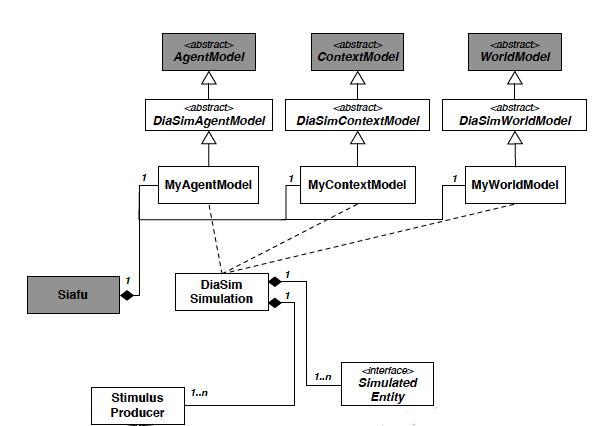
\includegraphics[width=\linewidth]{gfx/Chapter2/diasim_and_siafu}
	\caption{DiaSim and Siafu}
	\label{fig:diasim_and_siafu}
\end{figure}

I am considering to further analyze Siafu as a possible corner stone for our approach.\\

%Simact
SIMACT \ref{sec:simact}, is a flexible 3D smart home infrastructure simulator, developed in Java, specifically designed to help researchers working in the field of activity recognition. The simulator is released as open-source \cite{bouchard:simact:Online} under GPLv3 \cite{gpl:v3}.\\

The novel thing in this simulator is that entire scenarios and interactions can be designed only by using scripts and visual editors, without having to write one line of code. For the 3D design, they have used a modeling tool for house design and interior accessories from Google called SketchUp \cite{sketchup:online}. This comes with a great advantage as SketchUp's community maintains a huge library of free 3D models, where one can find almost any accessory that would fit in a home.\\

SIMACT provides a powerful and reusable simulation environment, with a strong platform, worth considering as basis for the simulator I am targeting to develop. My only concern is that I have not been able to determine the complexity of adding support for device simulation, as the main target of SIMACT is interaction with the physical environment. In conclusion, I will allocate some time during the system design process to analyze in detail if building on top of SIMACT would be possible.\\

%Simulation of Smart Environments
In the simulation of smart environments \ref{sec:sim_of_smart_envs}, the eHomeSimulator has an architecture providing loose coupling between components. Also, the underlying framework's architecture offers great support for reusability of services and integration with real-life devices. The devices are trivial, offering basic interactions (e.g. on/off) and they are static (the agent can't move them). Actually, all the agent can do is move around between some given bounds and interact with some of the device. There is no support for mobility of devices and wearable device, nor is it in plan for future work. Moreover, the representation of the agent is in 2D where he can be facing 4 directions, offering no support for various states like sitting, standing etc.\\

The project is close sourced, making it impossible to extend, to reuse or to contribute to it. In conclusion, there are a few lessons to be learnt from the architectural choices made within this project.\\

%Tatus
In Tatus \ref{sec:tatus}, the context-awareness is limited to sensors and actuators reacting to the user's position. This is actually not that bad because in the game engine SDK the developer can extract the position of entities, determine proximity of other entities within a given radius and determine the presence of other entities within a field of view. All these data helps to implement simulations for a wide range of sensors.\\

The user control provided by the game engine is pretty advanced allowing the agent to move in any direction, crouch, jump, sit etc. This is a big plus as it adds a good sense of reality to the game.\\

Multiple users can join and experience the same simulated environment at the same time. Not all players have to be human, non-player-characters (controlled by the AI of the engine) can be present as well.\\

One of the main challenges in developing the simulator was that the learning curve of the SDK, in order to extend it, was difficult and time-consuming. But, as a result, they have tried to provide a flexible simulation environment where researchers can easily simulate other environments without the need to modify any SDK level code.\\

Unfortunately the simulator is not open-source so making it unusable for research outside the institution it was developed in.\\

%Ubiwise
Although UbiWise \ref{sec:ubiwise} was released under LGPL\cite{lgpl}, offering the software to the open-source community, it presents two main issues from the perspective of my work. The first aspect is that it is oriented towards emulating device protoypes making it hard to emulate custom sensors. The second challenge is the learning curve it takes to get started with it. In order to customize it to a certain area, one would need to dive deep into the Q3A engine code, which is hard, tedious and time consuming task.\\
%END: DISCUSSION